\documentclass{standalone}


\begin{document}

\section[DNetPRO Implementation]{Algorithm implementation}\label{implementation}

The DNetPRO algorithm is made by a sequence of different steps which have to be performed sequentially for a signature extraction.
For this purpose each step can be optimized independently using the full set of available computational resources\footnote{
Further optimization can be performed in a cross validation environment and they will be discussed later in this section.
}.
In this section will be analyzed each part of the pipeline focusing on the optimization strategies used for the algorithm implementation.

The full code is open source and available at~\cite{DNetPRO}.
The code installation is automatically tested using \emph{travis} (for Linux and MacOS environments) and \emph{appveyor} (for Windows environments) at every commit.
The installation can be performed using \emph{CMake} or \emph{Makefile} and a full set of installation instructions can be found in the on-line project documentation.

The Python version of the algorithm (see next sections) can be installed via \emph{setup.py} and the compilable parts of it checked via \emph{CMake} or \emph{Makefile}.
The Python installer provides also the full list of dependencies of the project which will be automatically installed by the main.

In the Github repository can be found also a full list of example scripts and utilities to obtain the results shown in the next sections.
The complete benchmark pipeline can be found which can be run on cluster environment using the SnakeMake version of it (see next section).


\subsection[Pairs evaluation]{Combinatorial algorithm}\label{implementation:couples}

The most computational time expensive step of the algorithm is certainly the couples evaluation.
From a computation point-of-view this step requires $(O(N^2))$ operations for the full set of combination.
Since we want to perform also an internal Leave-One-Out cross validation for the couple performances estimation we have to add a $(O(S-1))$ to the algorithmic complexity.
Let's focused on some preliminary considerations before the implementation discussion:

\begin{itemize}

\item \textbf{Performances:} we aim to apply our method on large datasets since we have to focused on time performances of the code and particularly on this step (identified as bottleneck).
To reduce as much as possible the call stack inside our code we should perform the entire code with the small number of functions as possible and possibly inside a unique main.
Moreover we can simplify the for loop and take care of the automatic code vectorization performed by the optimizer at compile time (SIMD, \emph{Single Instruction Multiple Data}).
A further optimization step to take in count is related to the cache accesses: the use of custom objects inside the code should benefit from cache accesses (AoS vs SoA, \emph{Array of Structure} vs \emph{Structure of Arrays}).

\item \textbf{Interdependence:} the variable couple performances evaluation is a completely independent computational process and can be faced on as $N^2$ separately tasks.
Thus it can be easily parallelizable to increase speed performance.

\item \textbf{Simplify:} the use of simple classifier for performance evaluation simplify the computation and the storage of the relevant statistical quantities.
In the discussed implementation we focused on a Diag-Quadratic classifier (see Appendix A for further informations) and only means and variances of the data plays a role in its evaluation.

\item \textbf{Cross Validation:} the use of Leave-One-Out cross validation allows to perform substantially optimizations in the statistical quantities evaluations across the folds (see discussion in Appendix A - Numerical Implementation).

\item \textbf{Numerical stability:} we have also to take in care the numerical stability of the statistics since we are working in the assumption of a reasonable small number of samples compared to the amount of variables.
This behavior particularly affects the variance estimation: the chose of a numerical stable formula for this quantity play a crucial role for the computation because the classifier score has to be normalized by it.

\end{itemize}

With these idea in mind we can write a C++ code able to optimize this step of computation in a multi-threading environment with the purpose of testing its scalability over multi-core machines.

Starting from the first discussed point we chose to implement the full code inside a unique main function with the help of only a single SoA custom object and one external function (\emph{sorting algorithm} discussed in the next section).
This allows us to implement the code inside a single parallel section reducing the time of thread spawns.
We chose to import the data from file in sequential mode since the I/O is not affected by parallel optimizations.

Following the instructions suggested in Appendix A - Numerical Implementation we compute the statistic quantities on the full set of data before starting the couples evaluation.
Taking a look to the variance equation

$$
\sigma^2 = \frac{\sum_{i=1}^{S}(x_i - \mu)^2} {S - 1} = \frac{\sum_{i=1}^{S}({x_i}^2)} {S - 1} - \mu^2
$$
\\
we can see that the first equation involve the computation of the mean as a simple sum of the elements but a large number of subtractions from it that are numerical unstable for data outliers (moreover because they are elevated to square).
The better choice in this case is given by the second formulation that allows us to compute the both quantities in the formula inside a single parallel loop\footnote{
  To facilitate the SIMD optimization the code is written using only float (single precision) and integer variables.
  This precaution takes in care the register alignment inside the loops and facilitate the compile time optimizer.
}.
At each cross validation we will use the two pre-calculated sums of variables removing the only data point excluded by the Leave-One-Out.
Another precaution to take in care is to add a small epsilon to the variance before its use at denominator inside the classifier function to prevent numerical underflow.

The main role is still given by the couples loop.
The set of pair variables can be obtained only by two nested for loops in C++ and naive optimization can be obtained by simply reduce the number of iterations following the triangular indexes of the full matrix (by definition the score of the couple $(i, j)$ is equal to the score of $(j, i)$).
This precaution easily allows the parallelization of the external loop and drastically reduce the number of iteration but it also creates a link between the two iteration variables.
The new release of OpenMP libraries~\cite{OpenMP}\footnote{
  The OpenMP library is the most common non-standard library for C++ multi-threading applications.
} (from OpenMP 4.5) introduce a new \emph{keyword} of the language that allows the collapsing of nested for loops in a single one (whose number of iterations is given by the product of the single dimensions) in the only exception of completely independences of iteration variables.
So the best strategy to use in this case is to perform the full set of $N^2$ iterations with a single \textsf{collapse} clause in the external loop\footnote{
  Obviously the iteration where the inner loop variable is lower than the outer one will be skipped by an if condition.
}.

\lstset{style=snippet}
\begin{lstlisting}[language=Python, caption=Python parallel couples evaluation algorithm, label=code:py_couples]
import pandas as pd
import itertools
import multiprocessing

from sklearn.naive_bayes import GaussianNB
from sklearn.model_selection import LeaveOneOut, cross_val_score

def couple_evaluation (pair):
  f1, f2 = pair
  samples = data.iloc[[f1, f2]]
  score = cross_val_score(GaussianNB(), samples.T, labels,
                          cv=LeaveOneOut(), n_jobs=1).mean() # nested parallel loops are not allowed

  return (f1, f2, score)

def read_data (filename):
  data = pd.read_csv(filename, sep='\t', header=0)
  labels = data.columns.astype('float').astype('int')
  data.columns = labels

  return (data, labels)

if __name__ == '__main__':

  filename = 'data.txt'

  global data, labels
  data, labels = read_data(filename)

  Nfeature, Nsample = data.shape

  couples = itertools.combinations(range(0, Nfeature), 2)

  nth = multiprocessing.cpu_count()

  with multiprocessing.Pool(nth) as pool:
    score = zip(*pool.map(couple_evaluation, couples))

\end{lstlisting}

In this section we also provide an \quotes{equivalent} Python implementation with the use of common machine learning libraries and parallel settings (ref.~\ref{code:py_couples}).
In the next sections we will discuss the computational performances of this naive implementation with C++ one discussed above.



\subsection[Sorting]{Pair sort}\label{implementation:sort}

The sorting algorithm starts at the end of variable couple evaluation and re-order the pairs in ascending order to ease the next steps of signature identification\footnote{
  Up to now we are talking about couples performances meaning the classification accuracy of the feature pair.
  In some cases the simple accuracy is useless, especially when we are working with unbalanced population classes.
  In this case we can use a statistical score which takes in count the balanced between the right classifications of our samples (e.g Matthews Correlation coefficient, MCC).
  The developed code evaluate either the global accuracy of classification either the MCC and, with slight changes allows to perform the re-ordering of feature pair according to the desired score.
  Since in the next section we will discuss the application of the DNetPRO algorithm to real data using only the classification accuracy as score, we focused only on it in the next sections.
}.
This step is performed in the same code (and same parallel section) of the before section but it deserves an own topic for a better focus on the parallelization strategy chosen.
Moreover there are many common parallel implementation of sorting algorithm and to reach the best performances we have to chose the appropriated one.

The sorting algorithm are already implemented in serial version in the major part of the languages (Python and C++ included).
The naive version of the algorithms are also quite optimized and they perform the computation with complexity $(O(N\dot\log(N)))$\footnote{
  We are considering only un-stable sort in which the preserving order of equivalent elements in the array is not guaranteed.
}.
In this case we have not to re-invent any sorting technique but only insert as well as possible these algorithms inside a parallel sections and use the variable format chosen for couple performances storage.
Since we are working with SoA objects we need to re-order all the structure arrays in the same way.
So we can not use the a simple sort function but can compute the set of indexes that allow the re-order of the arrays, the so called \textsf{argsort} method.
To rearrange the indexes according to a given array of values we can use the templates in C++.

% insert image merge-sort here

As parallelization strategy we can yet invoke the new \emph{keywords} of OpenMP libraries and apply a \emph{divide-and-conquer} architecture using a tree of independent \emph{tasks}\footnote{
  Tasks in OpenMP are code blocks that the compiler wraps up and makes available to be executed in parallel.
}.
Using the maximum power of two of the available threads we split the computation in equal size sub-arrays and perform independent \textsf{argsort}s.
Then, going backwards to the subdivisions at each step we merge the sub-arrays two-by-two until the root.


\subsection[Network Signature]{Network signature}\label{implementation:network}

After the rearrangement of feature pairs in ascending order we can start to create the variable network and looking for its connected components as putative signatures.
Each feature will be represent a node in the network and a given pair will be a connection between them.
Since the full storage of the network would require a matrix $(N\times N)$ we have to chose a better strategy for the processing\footnote{
  We are working in the hypothesis of very large $N$.
}.

The ordered set of couples computes in the previous section represents a so-called \emph{COO sparse matrix} (Coordinate Format sparse matrix) and we can reasonable assume that the desired signature will be composed by the top ranking of them.
So, the first step will be to cut a reasonable percentage of the full set of pairs and process only them.

Moreover we are interested in a small set of variables unknown a prior.
The load of all the node pairs into the same graph can slow down the computation.
An iterative method (with stop criteria) can perform better in the large case of samples and only in worst cases the full set of pair will be loaded.

Since the described algorithm step does not require particular performance efficiency now, the main code used in our simulation was written in pure Python.
A C++ implementation of the same algorithm was developed with the help of the Boost Graph Library~\cite{BGL} (BGL) but to not overweight the code installation was reserved just for a style exercise.
In this section we discuss about this second version and about the strategies chosen to implement an efficiency version of it.
This version of the algorithm was also used as stand alone method for other applications that will be presented later.

BGL is a very wide framework for graph analysis based on template structures.
The library efficiency discourage the users to re-implement the same algorithms and for the current purposes it was resulted more than sufficient.

Starting from the top scorer feature pairs we progressively add each couple of nodes to an empty graph.
At each iteration step the number of connected components is evaluated until a desired number of nodes (greater or equal) is not reached\footnote{
  This procedure is quite similar to put a threshold value on the couple performances or just simpler highlight inside the full network the components linked by weights greater than a given value.
}.
Two degree of freedom are left to the user: in order, \textsf{pruning} and \textsf{merging}.
The first one perform an iteratively remotion of nodes with degree equal (or lower) than 1, i.e pendant nodes, until the graph core is not filtered.
The \textsf{merging} clause choose between the biggest connected component or the the set of all the disjoint connect components as putative signature.
The output of \textsf{merging} step determine the number of nodes in the graph which have been considered for the stop criteria.

A crucial role in the optimization of the algorithm is played by the BGL graph structure chosen.
Since the two degree of freedom imply a continuous rearrangement of the graph nodes the strategy chosen is to apply a filter mask over the main graph structure that highlights the only part of interest.
This can be done using the \textsf{boost :: filtered\_graph} object of BGL.
In ~\ref{code:featuresel} the C++ snippet is shown.

\lstset{style=c++}
\begin{lstlisting}[language=C++, caption=DNetPRO signature extraction, label=code:featuresel]
#include <boost/graph/adjacency_list.hpp>
#include <boost/graph/connected_components.hpp>
#include <boost/graph/filtered_graph.hpp>
#include <boost/function.hpp>
#include <boost/graph/iteration_macros.hpp>

typedef typename boost :: adjacency_list< boost :: vecS, boost :: vecS, boost :: undirectedS, boost :: property< boost :: vertex_color_t, int >, boost :: property < boost :: edge_index_t, int > > Graph;
using V = Graph :: vertex_descriptor;
using Filtered = boost :: filtered_graph < Graph, boost :: keep_all, boost :: function < bool(V) > >;


std :: vector < int > FeatureSelection (int ** couples, const int & min_size, bool pruning=true,  bool merging=true)
{
  Graph G;
  std :: vector < V > removed_set;
  Filtered Signature (G, boost :: keep_all {}, [] (V v) {return removed_set.end() == removed_set.find(v);});

  int L = 0, leave, Ncomp, i = 0;

  while ( true ){

    boost :: add_edge (couples[i][0], couples[i][1], G);

    while ( pruning ){

      leave = 0;
      BGL_FORALL_VERTICES (v, Signature, Filtered);
        if ( boost :: in_degree (v, Signature) < 2 ){
          removed_set.insert (v);
          ++ leave;
        }

      if ( leave == 0 )
        break;
    }

    if ( num_vertices (G) - removed_set.size() ){

      components.resize (num_vertices (G));

      Ncomp = boost :: connected_components (Signature, &components[0]);

      if ( merging ){

        BGL_FORALL_VERTICES (v, Signature, Filtered)
          core.push_back ( static_cast < int >(v) );
      }
      else {

        std :: map < int, int > size;
        for ( auto && comp : components ) ++ size[comp];

        auto max_key = std :: max_element (std :: begin(size), std :: end(size), [] (auto && p1, auto && p2) { return p1.second < p2.second; })->first;

        BGL_FORALL_VERTICES (v, Signature, Filtered)
          if ( components[v] == max_key )
            core.push_back( static_cast < int >(v) );
      }

      components.resize (0);
      L = static_cast < int >(core.size());
    }

    removed_set.clear();

    if ( L >= min_size ) break;

    ++ i;

    core.resize (0);
  }

  return core;
}

\end{lstlisting}

From the above description should be clear that given any set of ordered (in ascending order) couples of variables, this algorithm allows to extract the core network independently by the procedure which generate them.
So it can be used as dimensionality reduction algorithm of general purpose network structures.
An example of this kind of application was reported in Appendix B - Venice Road Network in which we summarized the results of~\cite{Mizzi2018, CurtiSDPS2018}.


\subsection[Python wrap]{DNetPRO in Python}\label{implementation:python}

Up to now we are focusing on the algorithm performances leaving out the usability of the DNetPRO algorithm for the (research) community.
Despite the C++ is one of the most efficient and old programming language\footnote{
  Still in common use in scientific research groups.
}, the Python language users are increasing in the last few years.
Python is becoming leader in scientific research publications and the large part of Machine Learning analysis are performed using Python libraries (in particular \emph{scikit-learn} library).
So we have to reach a compromise between the performances and usability of new developed codes and it can be reached using the Cython~\cite{behnel2010cython} framework.

Cython \quotes{language}\footnote{
  It is not a real programming language since it is based on Python.
  However it has its own syntax and keywords which are different either from Python either from C++.
  In the end it needs a compiler to run and it is certainly different from Python.
} allows an easy interface between C++ codes and Python language.
With a relatively simple wrapping of the C++ functions they can be used inside a pure Python code preserving as much as possible the computational performances of the pure C++ version.
In this way we can create a simple Python object which performs the full set of DNetPRO steps and moreover which is compatible with the functions provided by the other machine learning libraries.

With this purposes we chose to operate a double wrap of the C++ functions to separate as much as possible the C++ component from the Python one\footnote{
  Cython wrap are very powerful tools for C++ integration into Python code but, by experience, they are difficult to manage by pure-Python users.
  A simple workaround is to perform a first wrap of the C++ function inside a Cython object and a second wrap of it into a pure-Python one.
  This two-steps wrap certainly gets worse the computational performances but it allows a complete separation between the compiled part of the code (Cython) and the interpreted (Python) one.
  Moreover we can leave back all the checks on input parameters
  in the C++ version since they will be performed at run time in the Python wrap.
}.
The Python object was written considering a full compatibility with the \emph{scikit-learn} library to allow the use of the DNetPRO feature selection as an alternative component of other Machine Learning pipelines.


\subsection[Pipeline]{DNetPRO in Snakemake}\label{implementation:snakemake}

The starting (silent) hypothesis done until now is that we are running the DNetPRO algorithm on a single dataset (or better on a single Hold-Out subdivision of our data).
On this configuration it is legal to stress as much as possible the available computational resources and parallel processing each step of the algorithm.

If we want introduce our algorithm inside a larger pipeline in which we compare the resulting obtained over a Cross-Validation of our datasets we have to re-think about the parallelization done.
In this case each fold of the cross validation can be interpreted as independent task and following the main programming rule \emph{\quotes{parallelize the outer, vectorize the inner}} we should spawn a thread for each fold and perform the couple evaluation in sequential mode.
Certainly, the optimal solution would be to separate our jobs across a wide range of inter-connected computers and still perform the same computation in parallel but it would required to implement our hybrid (C++ and Python) pipeline in a Message Passing Interface (MPI) environment.

An easier solution to overcome all these problems can raise by the use of SnakeMake~\cite{snakemake} rules.
SnakeMake is an intermediate language between Python and Make.
Its syntax is almost like the Make language but with the help of the easier and powerful Python functions.
It is wide use for bioinformatic pipeline parallelization since it can easily applied over single or multi-cluster environment (master-slave scheme) with a simple change of command line.

\begin{center}
\begin{figure}[htbp]
\centering
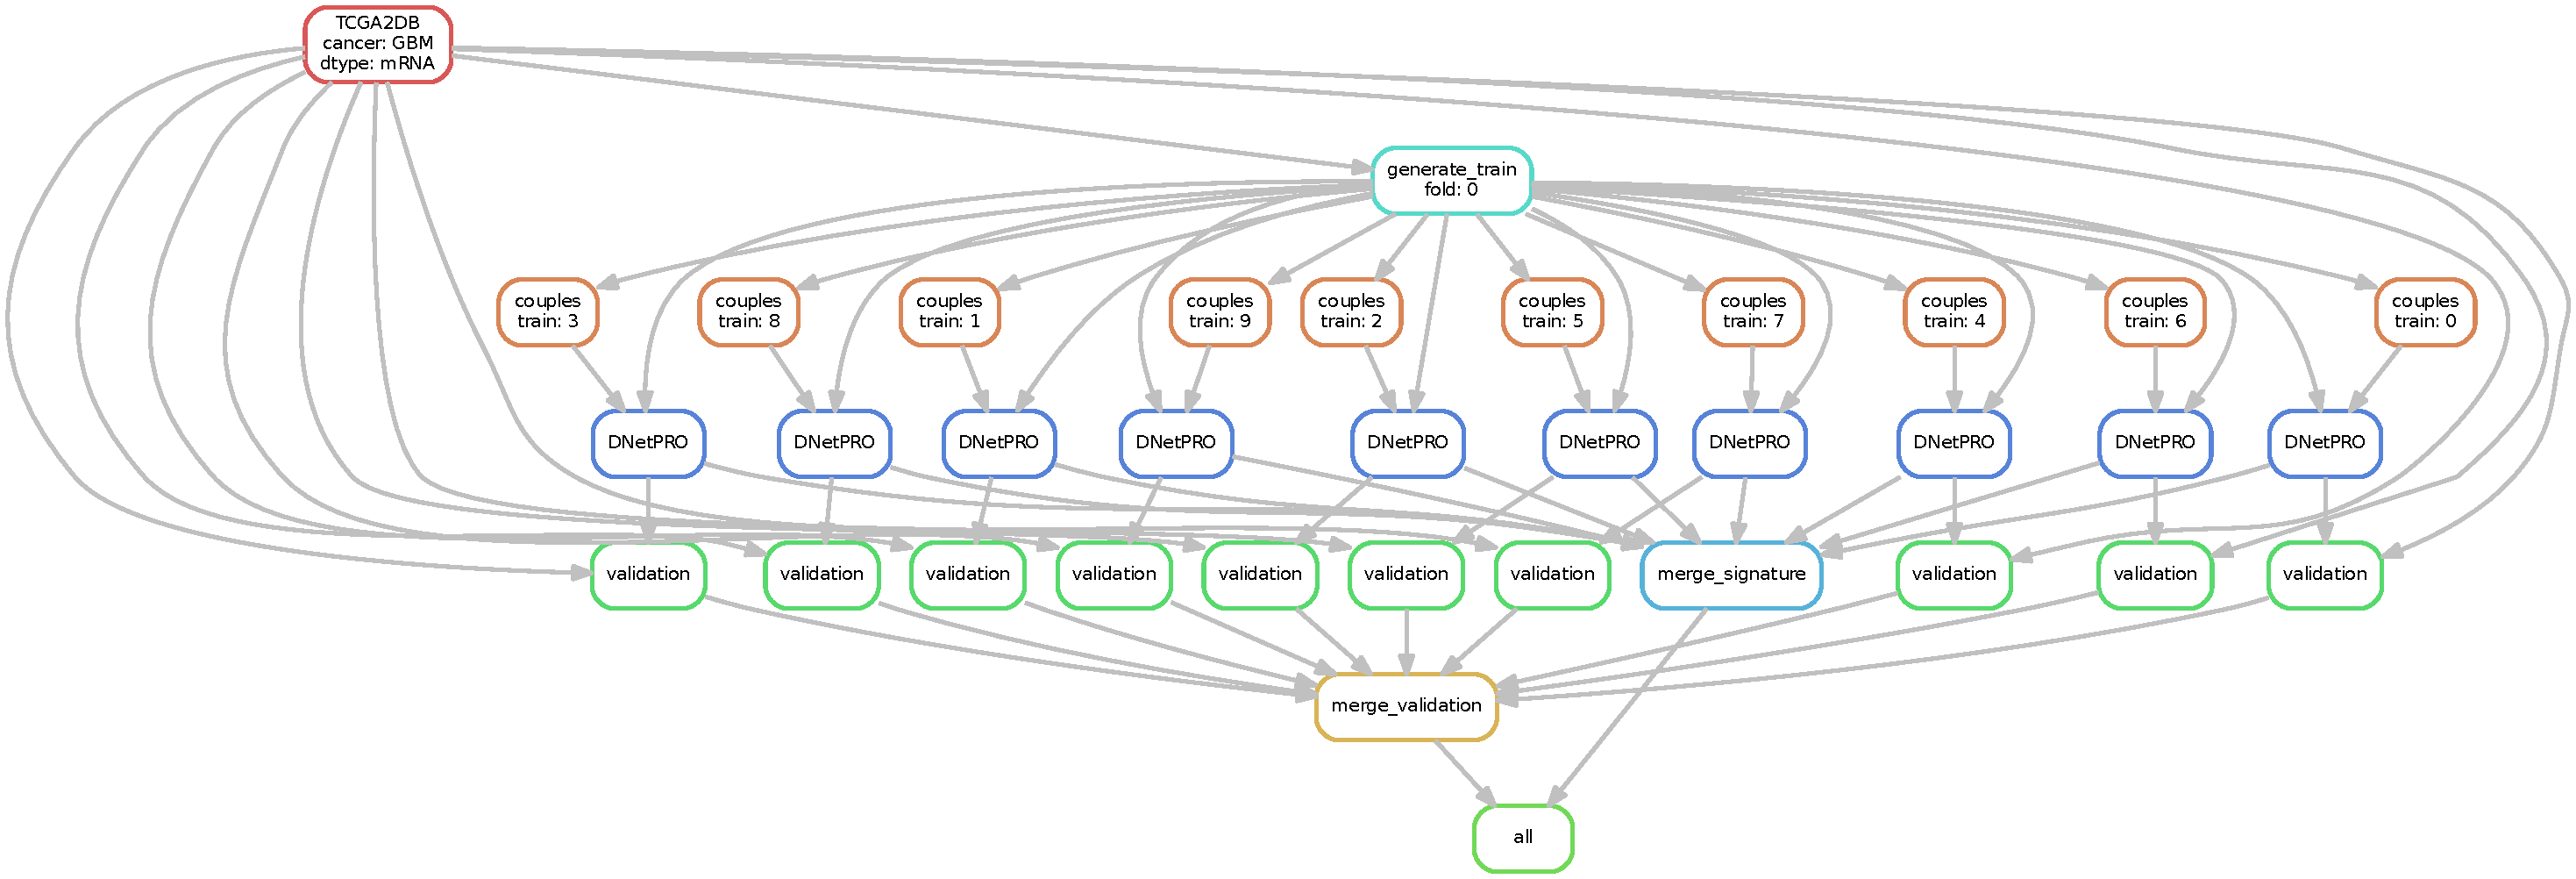
\includegraphics[width=0.85\textwidth]{qdanet_pipe_single.pdf}
\caption{Example of DNetPRO pipeline on a single cross validation.
It is highlighted the independence of each fold from each other.
This scheme shows a possible distribution of the jobs on a multi-threading architecture or for a distributed computing architecture.
The second case allows further parallelization scheme (hidden in the graph) for each internal step (e.g. the evaluation of each pair of genes).
}
\label{fig:dnet_workflow}
\end{figure}
\end{center}

So to improve the scalability of our algorithm we implement the benchmark pipeline scheme using Snakemake rules and a work-flow example for a single cross-validation is shown in Fig.~\ref{fig:dnet_workflow}.
In this case each step of Fig.~\ref{fig:dnet_workflow} can be performed by a different computer unit preserving the multi-threading steps, with a maximum scalability and the possibility to enlarge the problem size and the number of variables.



\subsection[Time performances]{Time performances}\label{implementation:timing}


%Description of the algorithm implementation in C++.
%Parallelization of the algorihtm.
%Use of BGL for network processing (filter node using view)
%Wrap in Python for Sklearn use
%Time Performances on different machines.


\end{document}